
\documentclass{article}

\usepackage[utf8]{inputenc}

\usepackage{amsmath, bm}
\usepackage{graphicx}
\usepackage{amssymb}
\usepackage{float}
\usepackage{caption}
\usepackage{subcaption}
\usepackage{hyperref}
\usepackage{tikz}
\usepackage{layout}


\begin{document}


Objectives of Prepatory work
\begin{itemize}
    \item To understand the functioning of a propellor by reading on propellor theory, actuator discs, blade element method, and lifting line theory.
    \item To understand the acoustics, read up on theory of sound, the noise generated by turbulent flows and airfoils.
\end{itemize}


\section{METHOD OF CALCULATING PERFORMANCE OF DUAL-ROTATING PROPELLERS FROM AIRFOIL CHARACTERISTICS By Irven Naiman}

\subsection{Assumptions}

\begin{itemize}
    \item The oscillating induced-velocity field may be replaced by a uniform field, the value for which is equal to the mean value of the oscillating field.
    \item The mean value of the induced velocity is taken to be F times the value induced at the vortex sheet. This is a correcting factor for finite number of blades.
    \item Because the general solution for the duel propeller is lacking, the self-induced velocities are determined in the same way as for a single propeller, that is, the value of F is that for a single propeller.
    \item The propellers are assumed to be sufficiently close together that changes in axial velocity between them are negligible.
\end{itemize}

\subsection{Form of General Problem}

Need to determine lift and drag on a propeller from geometry (number of blades, airfoil section, solidity [$\sigma$], and blade-angle setting [Twist]) at a known value of the advance diameter ratio.

The correct resolution of the lift and drag into thrust and torque requires that the direction of inflow velocities, or the pitch angle of the vortex sheet, $\phi$ to be known.

The lift coefficient is a function of the angle of attack

\begin{equation}
    C_L = K\alpha = K(\theta - \phi)
\end{equation}

The loading of the propeller is a function of the pitch and magnitude of the induced velocities of the vortex sheet, as shown by Goldstien \ref{Goldstien}
\begin{equation}
    \sigma C_L = 4F \sin(\phi)\tan(\epsilon)
\end{equation}

Where $ F = \frac{K}{\cos^2(\phi)} $ and $ \tan(\epsilon) = \frac{w}{W} $, $\phi$ is the pitch angle of vortex sheet.

$w$ is the induced velocity normal to the vortex sheet, and W is the resultant velocity of the blade element along the sheet.

\begin{figure}[H]
    \centering
    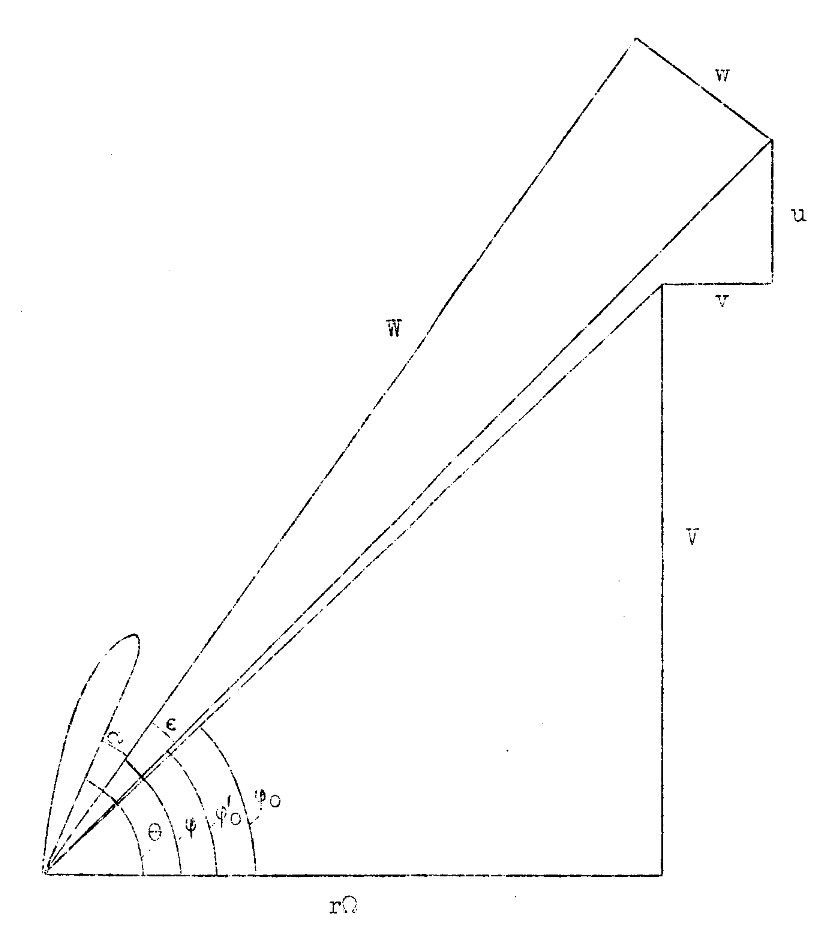
\includegraphics[width=0.5\textwidth]{irven_vel_diagram.jpg}


\end{figure}


The general propeller equation may therefor be written
\begin{equation}
    \Phi(\theta,\psi,\psi_0) = M(\theta - \phi) - \frac{4F}{\sigma} \sin \phi \tan (\phi - \phi_0) = 0
\end{equation}

If the propeller is working not in free air but in an air stream that has been modified by body interference, body wake, or slipstream of another propeller,the advance angle $\phi_0'$ appropriate to these conditions must be used instead of $\phi_0$.

Further extension to dual propellers is not of interest.

\end{document}



